\chapter{معرفی}
\label{chapter:introduction}

 در این فصل ابتدا با کدگذاری اندیس، کاربردها و تاریخچه‌ی آن آشنا می‌شویم. سپس به کدگذاری اندیس منعطف پرداخته و با تاریخچه‌ی پژوهشی آن آشنا می‌شویم. در بخش پایانی این فصل نیز پس از بررسی اهداف و دست‌آوردهای پژوهشی، ساختار این پایان‌نامه را شرح می‌دهیم.
\pagebreak

\section{مقدمه}
کدگذاری اندیس(که از این پس، به اختصار آن را با
\icod
نمایش می‌دهیم) در سال ۱۹۸۸ توسط 
\transf{بیرک}{Birk}
و
\transf{کول}{Kol}
هنگام بررسی ارتباطات ماهواره‌ای در
\cite{25}
معرفی شد. پس از آن \icod کاربردهای متعددی در مسائل مختلف نظری و عملی پیدا کرد. این موضوع باعث شده است تا طی دو دهه‌ی گذشته ابزارهای مختلفی از بخش‌های مختلف ریاضی، مانند نظریه‌ی گراف، نظریه‌ی کدگذاری و نظریه‌ی اطلاعات در توسعه‌ی این مبحث مورد استفاده قرار گیرند. \icod منشا مسئله‌های گوناگونی است. مسائل مختلفی با کاربرهای گوناگون از این مسئله نشئت گرفته اند. یکی از این مسائل کدگذاری اندیس منعطف است، که موضوع اصلی این پایان‌نامه است.

	\icod، یک مسئله‌ی
\transf{\nphard}{NP-Hard}
است و در نتیجه امیدی به حل آن در زمان چندجمله‌ای، در حالت کلی نیست. به همین دلیل پژوهشگران با تغییر پارامترهای مسئله و ایجاد مسائل جدید سعی در حل این مسئله تحت شرایط مختلف کرده‌اند. کدگذاری اندیس منعطف که موضوع این پایان‌نامه است نیز با کاهش سختگیری شرایط مدگذاری اندیس ایجاد شده است، اما همان‌طور که در فصل سوم خواهیم دید، این مسئله نیز
\nphard
است. همان طور که با توسعه‌ی کدگذاری اندیس، به کدگذاری اندیس منعطف رسیدیم، می‌توانیم برای  این مسئله نیز توسعه‌های متنوعی با کاربرهای متفاوت در دنیای واقعی ایجاد کنیم.

به دلیل اهمیت \icod، در این فصل ابتدا به بررسی آن می‌پردازیم. با تاریخچه تحقیقاتی، کاربرها و اهمیت آن در صنعت و تعریف دقیق آن آشنا می‌شویم. سپس با توسعه آن، به مسئله‌ی اصلی این پایان‌نامه، یعنی کدگذاری اندیس منعطف می‌رسیم. معرفی \icod از آن جهت حائز اهمیت است که باعث روشن‌تر شدن فضای مسئله‌‌ی اصلی و ریشه‌های آن می‌شود و دلیل این‌که چرا گونه‌های مختلفی برای این مسئله ایجاد شده است را روشن می‌کند.
\pagebreak
\section{کدگذاری اندیس}
\subsection{
	معرفی \icod
	}
	\begin{wrapfigure}{l}{0.4\textwidth}
		\centering
		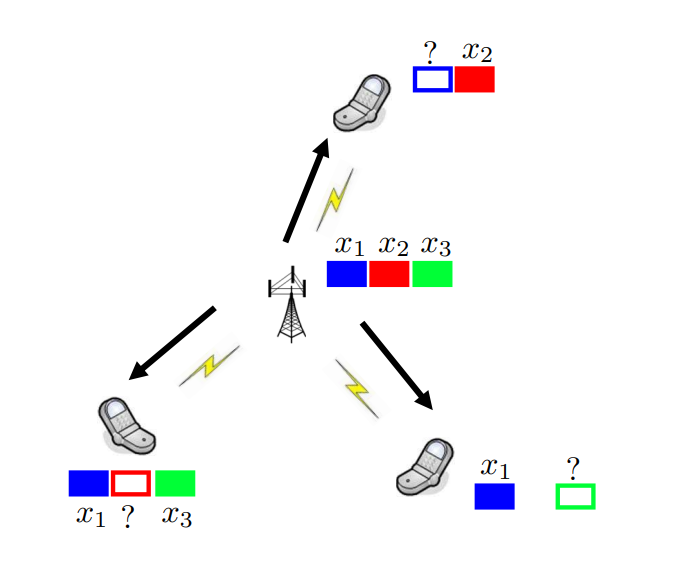
\includegraphics[width=1\linewidth]{figs/chapter1/fatemeh1}
		\caption[
					ماهواره‌ای در حال ارسال پیام به سه گیرنده
		]{
			ماهواره‌ای در حال ارسال پیام به سه گیرنده
			\cite{fatemehbook}
		}
		\label{fig:fatemeh1}
	\end{wrapfigure}
با یک مثال، \icod را معرفی می‌کنیم. فرض کنید مطابق 
\autoref{fig:fatemeh1}،
یک ماهواره‌‌ی رسانه‌ای در حال 
\transf{ارسال}{broadcast, transmit}
 اطلاعات برای سه گیرنده‌ی مختلف است. 
هر گیرنده، با توجه به موقعیت مکانی خود (برای مثال داشتن ارتباطات دیگر با منابع خبری مانند روزنامه‌ی محلی و \ldots) از تعدادی از خبرهای روز مطلع است و به دنبال یک خبر جدید است که از آن اطلاعی ندارد. ماهواره در هر لحظه می‌تواند یکی از خبرهای روز را از طریق امواج به سمت کره‌ی زمین ارسال کند، در این صورت تمام گیرنده‌ها آن خبر را دریافت خواهند کرد (علاوه بر این ممکن است به جز گیرنده‌های مورد نظر ما، شنودگری نیز در تلاش برای بازیابی اطلاعات باشد، برای بررسی این حالت به
\autoref{sec:privatepliable} 
رجوع کنید.) اگر به گیرنده‌ای خبری برسد که آن را از پیش می‌داند یا به هر دلیلی به دنبال آن نیست، باید صبر کند تا خبر مورد نظر خود را دریافت کند. 

	\begin{wrapfigure}{l}{0.4\textwidth}
	\centering
	\begin{tikzpicture}[->, >=stealth, auto, semithick]
		% Set the positions of the nodes
		\node[circle, draw=blue, fill=blue!20, inner sep=0pt] (C1) at (0,2) {$C_1$};
		
		\node[circle, draw=blue, fill=blue!20, inner sep=0pt] (C2) at (1.5,2) {					$C_2$				};
		\node[circle, draw=blue, fill=blue!20, inner sep=0pt] (C3) at (3,2) {$C_3$				};
		
		\node[circle, draw=green, fill=green!20, inner sep=0pt] (B1) at (0,0) {$B_1$};
		\node[circle, draw=green, fill=green!20, inner sep=0pt] (B2) at (1.5,0) {$B_2$};
		\node[circle, draw=green, fill=green!20, inner sep=0pt] (B3) at (3,0) {$B_3$};
			% Draw the edges
			\draw (C1) -- (B2);
			\draw (C1) -- (B3);
			\draw (C2) -- (B1);
			\draw (C2) -- (B3);
			\draw (C3) -- (B1);
			\draw (C3) -- (B2);
			\draw[color=red, dashed] (C1) -- (B1);
			\draw[color=red, dashed] (C2) -- (B2);
			\draw[color=red, dashed] (C3) -- (B3);
		
		% Position the parts
		\begin{scope}[on background layer]
			\node[fit=(C1) (C2) (C3), draw=blue, fill=blue!10, rounded corners] {};
			\node[fit=(B1) (B2) (B3), draw=green, fill=green!10, rounded corners] {};
		\end{scope}
	\end{tikzpicture}
	\caption[
	نمونه‌ای از \icod
	]{
		\centering
			نمونه‌ای از مسئله کدگذاری اندیس
			
		یال سیاه :اطلاعات قبلی گیرنده
		
		یال قرمز: پیام مورد نظر گیرنده‌
	}
	\label{first_example}
\end{wrapfigure}

برای نشان دادن یک \transf{نمونه}{instance}
از \icod، معمولا از یک نمایش گرافی استفاده می‌کنیم. برای مثال در 
\autoref{first_example}، 
 اگر گیرنده‌ها را با
$c_1$، $c_2$ و $c_3$
(حرف اول کلمه
\lr{client})
و خبرها را با
$b_1$، $b_2$ و $b_3$
(حرف اول کلمه
\lr{bit})
نشان دهیم گیرنده‌ی اول، خبر دوم و سوم را می‌داند و به دنبال \transf{بازیابی}{retrieve} خبر اول است. به طور مشابه گیرنده‌های دوم و سوم به ترتیب به دنبال بازیابی خبرهای دوم و سوم هستند. 

\noindent
سوالی که در این نمونه‌های \icod به دنبال آن هستیم این است که، کم‌ترین تعداد دفعات ارسال خبر از طرف ماهواره برای این‌که تمام گیرنده‌ها پیام مورد نظر خود را بازیابی کنند، چقدر است؟

برای مدل‌سازی ریاضی مسئله، خبرها را با متغیرهای تصادفی مدل می‌کنیم که از الفبای
$\chi$
می‌آیند. همچنین پیام‌های ارسال شده توسط ماهواره نیز اعضای همین مجموعه‌اند. به عنوان نمونه، در مثال بالا داریم:
$\chi = \mathbb{F}_2$
و
$X = (0, 0, 1)$.
یک راه‌حل برای مثال بالا این است که ماهواره خبر مورد نظر هر گیرنده را به ترتیب ارسال کند. یعنی اگر پیام‌های ارسالی ماهواره را با
$Y= (y_1, y_2, \ldots)$
نشان دهیم در این صورت ارسال
$Y = (0, 0, 1)$
توسط ماهواره باعث می‌شود تمام گیرنده‌ها به پیام مورد نظر خود برسند. در این ایده‌ی ابتدایی، باید به تعداد گیرنده‌ها(یا به تعداد پیام‌ها در صورتی که از تعداد گیرنده‌ها کم‌تر باشند) به ارسال پیام نیاز داریم.
 
راه دیگر این است که ماهواره مقدار
$Y = (y_1)$
که
$y_1 = x_1 + x_2 + x_3$
را ارسال کند. در این صورت گیرنده‌ی اول با در دست داشتن
$x_2$
و
$x_3$
و همچنین
$y_1$
که از ماهواره آن را دریافت کرده است، با استفاده از فرمول
$y_1 - x_2 - x_3$
می‌تواند خبر مورد نظر خود را به دست آورد. دو گیرنده‌ی دیگر نیز به طور مشابه با همین تک ارسال می‌توانند خبر مورد نظر خود را بازیابی کنند و در نتیجه تنها با یک بار ارسال پیام به جای ۳ مرتبه، ماهواره می‌تواند نیاز تمام گیرنده‌ها را برطرف کند.

در 
\icod،
$m$
متغیر تصادفی،
$n$
گیرنده و یک فرستنده داریم. هر گیرنده از قبل مقدار بعضی از متغیرها را می‌داند و به دنبال مقدار یک متغیر تصادفی دیگر است که مقدار آن را نمی‌داند.

برای نمایش مسئله از گراف‌های دوبخشی استفاده می‌کنیم. در یک بخش رئوسی متناظر پیام‌ها(متغییرهای تصادفی) و در بخش دیگر رئوسی متناظر گیرنده‌ها قرار می‌گیرند. به ازای هر گیرنده که یکی از متغییرها را می‌داند یک یال از راس متناظر گیرنده به راس متناظر متغییر می‌کشیم، مانند
\autoref{first_example}.

\icod، یافتن کم‌ترین تعداد ارسال لازم توسط فرستنده است، به طوری که تمام گیرنده‌ها اطلاعات مورد نیاز خود را بازیابی کنند.
	\subsection{تعریف رسمی کدگذاری اندیس}
در این بخش برای تعریف 
\icod
در حالت کلی و تعریف‌های اولیه دیگری که نیاز داریم، از فصل اول کتاب
\cite{fatemehbook}
استفاده می‌کنیم.
\begin{definition}[\icod]
	فرض کنید
	$n$
	گیرنده و
	$m$
	متغیر تصادفی به صورت
	$X_1, \ldots, X_m \in \mathbb{X}$
	داریم. همچنین گیرنده‌ی
	$i$-ام
	مقدار متغیرهای تصادفی‌ای که اندیسشان در مجموعه‌ی
	$S_i \subseteq [m]$
	آمده است را می‌داند.	به این مجموعه‌ها، مجموعه‌ی اطلاعات جانبی می‌گوییم. به چندتایی
	$(n, m, S =(S_1, \ldots, S_n) )$
	یک نمونه از
	\icod
	می‌گوییم.
\end{definition}
\begin{definition}[اندیس‌کد]
	\label{def:icod}
	برای یک نمونه‌ی \icod مانند
	$(n, m, S)$،
	یک
	$(t_1, \ldots, t_n, r)$
	-اندیس‌کد از اجزای زیر تشکیل می‌شود:
	\begin{itemize}
		\item 
      پیام‌ها:
		$n$
		 متغیر تصادفی که به آن‌ها پیام می‌گوییم. پیام
		  $i$-ام
            یک بردار 
		  $t_i$ تایی
            از الفبای
		  $\chi$
		  است. یعنی:
		  $x_i = (x_{i1}, \ldots, x_{it_i}) \in \chi^{t_i}$
		  \item
		  کدگذار:
		   یک تابع کدگذاری به شکل:
		   $\phi: \prod\limits_{i = 1}^n \chi^{t_i}  \rightarrow \chi^r$
		  \item
		  کدگشاها:
		  $n$
		  تابع کدگشا به شکل
		  $$\forall i \in [n]: \psi_i: \chi^r \times  \prod\limits_{j \in S_i} \chi^{t_j} \rightarrow \chi^{t_i}$$
		  به گونه‌ای که برای هر
		  $x^n \in \prod\limits_{i = 1}^{n} \chi^{t_i}$
		  داشته باشیم:
		  $$\forall i \in [n]: \psi_i(\phi(x^n), x[S_i]) = x_i$$
	\end{itemize}
\end{definition}

اگر بخواهیم به صورت شماتیک به تعریف بالا نگاه کنیم، همان‌طور که در
\autoref{fig:fatemeh2}
\begin{figure}
	\centering
	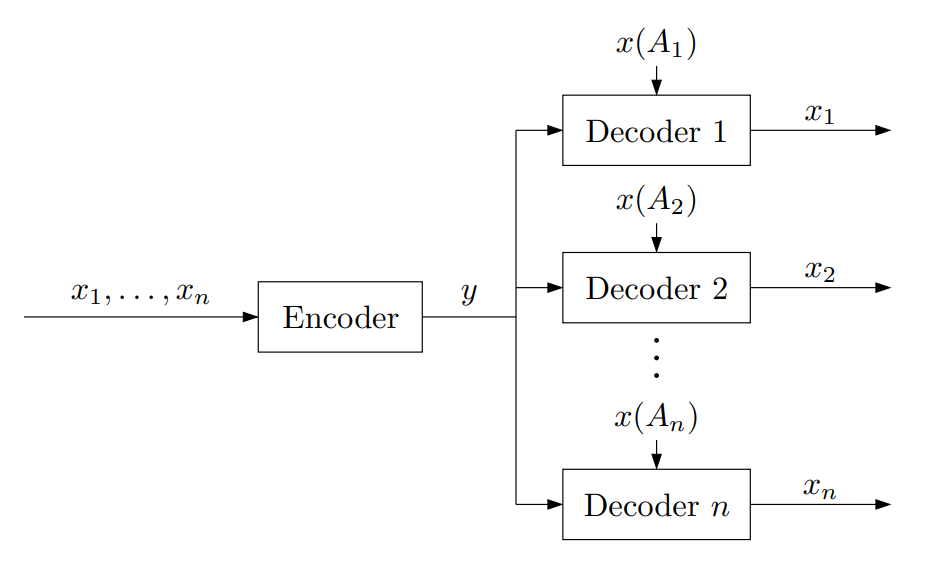
\includegraphics[width=0.7\linewidth]{figs/chapter1/fatemeh2}
	\caption[
		شمای کلی 
	\icod
	]{
		شمای کلی 
		\icod
	\cite{fatemehbook}\footnotemark
	}
	\label{fig:fatemeh2}
\end{figure}
	\footnotetext{در این کتاب از نماد
	$A_i$
	به جای
	$S_i$
	استفاده شده است.}
قابل مشاهده است، در یک نمونه از مسئله‌ی
\icod
فرستنده با ترکیب متغیرها به یک بردار
$Y$
می‌رسد و با ارسال آن به گیرنده‌ها به آن‌ها اطلاعاتی محدود و مشخص از مقدار متغیرها می‌دهد. سپس گیرنده‌ها بر اساس بردار دریافتی و اطلاعات جانبی خود به بازیابی اطلاعات می‌پردازند.

	به یک
	$(t, t, \ldots, t, r)$-اندیس‌کد،
	یک
	$(t, r)$-اندیس‌کد
	نیز می‌گوییم.
	
	اگر عمل‌های خطی روی الفبای
	$\chi$
	خوش‌تعریف باشند، برای مثال
	$\chi = \mathbb{F}_q$
	یا یک حلقه (برای مثال حلقه به 
	\cite{Connelly2018}
	مراجعه کنید) و توابع کدگذار و کدگشا همگی خطی باشند به این کد، کد خطی می‌گوییم. 
	\begin{definition}
		\label{def:linearcode}
	اگر 
	$\forall i \in [n]: t_i = 1$،
	کد اسکالر و در غیر این‌ صورت، کد برداری خواهیم داشت.
	\end{definition}
	برای مثال در 
	\autoref{fig:fatemeh1}
	با یک 
	$(1, 1, 1, 2)$-کد
	مواجه هستیم. اگر در این مثال الفبا را
	$\chi = \mathbb{F}_2$
	در نظر بگیریم، آنگاه توابع کدگذار و کدگشای زیر پاسخی برای مسئله‌اند:
	\begin{align*}
	\phi(X) &= (Y) \Rightarrow \phi(x_1, x_2, x_3) = (x_1 + x_2, x_3) \\
	\psi_1 &= y_1 + x_2, \psi_2 = y_1 + x_3, \psi_3 = y_2
	\end{align*}
	\begin{definition}[نرخ قابل دستیابی]
		به چندتایی مرتب
		$(R_1, \ldots, R_n) \in \mathbb{R}_{\geqslant 0}^n$
		نرخ قابل دستیابی برای \icod گوییم اگر یک 
		$(t_1, \ldots, t_n, r)$-اندیس‌کد
		 وجود داشته باشد که
		$$\forall i \in [n]: R_i \leq \frac{t_i}{r}.$$
		\end{definition}
  \begin{definition}[ناحیه ظرفیت]
  	به بستار مجموعه‌ی تمام نرخ‌های قابل دستیابی، ناحیه ظرفیت می‌گوییم و آن را با
		$\mathscr{C}$
		نشان می‌دهیم.
	\end{definition}
	
	هدف نهایی مطالعه کدگذاری، یافتن ساختار ناحیه ظرفیت در هر \icod و همچنین ساخت یک روش کدگذاری کارا برای دستیابی به نرخ‌های قابل دستیابی است.
	
	به صورت کلی بهینه‌سازی یک پارامتر نسبت به بهینه‌سازی هم‌زمان چند پارامتر ارجحیت دارد، برای همین می‌توان از روش دیگری برای نشان دادن ناحیه ظرفیت استفاده کرد.
	\begin{definition}[ناحیه ظرفیت جهت‌دار]
	برای بردار
	$\mu = (\mu_1, \ldots, \mu_n) \in \mathbb{R}_{\geqslant 0}^n $،
    ناحیه ظرفیت در جهت
	$\mu$
	را به صورت زیر تعریف می‌کنیم:
	$$C(\mu) = max \{R: R \mu \in \mathscr{C}\}$$
\end{definition}

\begin{remark}
	با کمک ناحیه‌های ظرفیت جهت‌دار می‌توان ناحیه ظرفیت را به شکل زیر بازنویسی کرد:
	$$\mathscr{C} = \bigcup\limits_{\mu} \{(R_1, \ldots, R_n): R_i \leq C(\mu) \mu_i, i \in [n]\}$$
	\begin{definition}[ظرفیت متقارن]
	ظرفیت متقارن را به صورت
	$C_{sym} = C(1) $
	 تعریف می‌کنیم.
	 \end{definition}
\end{remark}

از تعریف ظرفیت متقارن داریم:
$$C_{sym}= \sup\limits_{r} \sup_{(t, r)-code} \dfrac{t}{r} = \lim\limits_{r \rightarrow \infty} \sup_{(t, r)-code} \dfrac{t}{r} $$
که تساوی بین سوپریمم و لیمیت به دلیل زیرجمعی بودن
$$\sup_{(t, r_1 + r_2)-code} t \geqslant \sup_{(t_1, r_1)-code} t_1 + \sup_{(t_2, r_2)-code} t_2$$
و لم
\transf{فکته}{
\href{https://en.wikipedia.org/wiki/Subadditivity}{Fekete}}
به دست می‌آید.

حال می‌توانیم پارامتری تعریف کنیم که به جای بهینه‌سازی هم‌زمان چند پارامتر فقط یک پارامتر بهینه شود.
\begin{definition}
	نرخ انتشار به صورت زیر تعریف می‌شود:
	$$\beta = \dfrac{1}{C_{sym}}$$
\end{definition}
\begin{remark}
طبق تعریف داریم:
$$\beta = \inf\limits_{t} \inf\limits_{(t, r) codes} \dfrac{r}{t} = \lim\limits_{t \rightarrow \infty} \inf\limits_{(t, r) codes} \dfrac{r}{t}$$
همچنین به سادگی مشاهده می‌شود که:
	$$\dfrac{1}{n} \leq C_{sym} \leq 1, 1 \leq \beta \leq n$$
\end{remark}
تاکنون راجع به ناحیه ظرفیت به صورت کلی صحبت کردیم ولی ناحیه ظرفیت برای یک مسئله خاص وابسته به الفبای
$\chi$
انتخاب شده است، پس شاید به نظر برسد که بهتر است آن را به صورت
$\mathscr{C}_\chi$
نمایش بدهیم اما لم زیر نشان می‌دهد که این‌گونه نیست!
\begin{lemma}
	برای هر دو الفبای متناهی
	$\chi_1, \chi_2$
	داریم:
	$$\mathscr{C}_{\chi_1 }= \mathscr{C}_{\chi_2} $$
\end{lemma}
اثبات این لم در
\autoref{appendix:l1}
 آمده است.

\begin{notation}
		\label{notation:graph1}
	 با فرض مشخص بودن میدان متغیرها، هر نمونه از \icod توسط مجموعه‌های اطلاعات جانبی
	$S_1, \ldots, S_n$
	به صورت یکتا مشخص می‌شود. به صورت پیش‌فرض گیرنده‌ی
	$i$-ام
    به دنبال بازیابی پیام
	$i$-ام
 است مگر این‌که خلاف آن به صورت صریح گفته شود. پس دانستن مجموعه‌های اطلاعات جانبی برای مشخص کردن یک نمونه کافی است. اما نمایش‌های دیگری نیز برای مسئله کدگذاری اندیس وجود دارد. در واقع نمایش‌های متفاوت اطلاعات جانبی، زاویه دیدهای مختلفی نسبت به مسئله به ما می‌دهند. در ادامه ۲ نمایش مختلف را معرفی می‌کنیم:
\begin{itemize}

	\item
	برای هر گیرنده یک راس قرار می‌دهیم. اگر گیرنده‌ی
	$i$-ام
	پیام
	$x_j$
	را به عنوان اطلاعات جانبی داشته باشد، از راس
	$v_i$
	به راس
	$v_j$
	یک یال جهت دار می‌کشیم
	\autoref{fig:fatemeh3}.
 
	\begin{figure}[H]
		\centering
		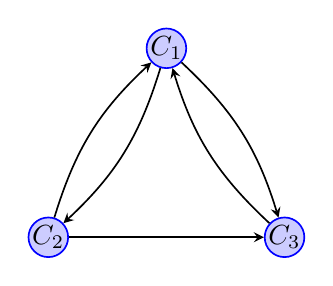
\begin{tikzpicture}[->, >=stealth, auto, semithick]
			% Set the positions of the nodes
			\node[circle, draw=blue, fill=blue!20, inner sep=0pt] (C1) at (0,0) {$C_1$};
			
			\node[circle, draw=blue, fill=blue!20, inner sep=0pt] (C2) at (-1.5,-2.4) {$C_2$};
			\node[circle, draw=blue, fill=blue!20, inner sep=0pt] (C3) at (+1.5,-2.4) {$C_3$};
			% Draw the edges
			\draw (C1) to[bend left=15] (C2);
			\draw (C1) to[bend left=15] (C3);
			\draw (C2)to[bend left=15] (C1);
			\draw (C2) to(C3);
			\draw (C3)to[bend left=15](C1);
		\end{tikzpicture}
		\caption{
			گراف اطلاعت جانبی برای مسئله
			\\
			$S_1 =	\{2, 3\}, S_2 = \{1\}, S_3 = \{1, 2\}$
		}
		\label{fig:fatemeh3}
	\end{figure}
	
این روش برای زمانی است که تعداد پیام‌ها و گیرنده‌ها برابر باشد. در حالت کلی ممکن است این‌طور نباشد و به علاوه، روش بالا درک مسئله را سخت‌تر می‌کند.
	\item 
 به جای گراف با
	$n$
	راس می‌توان از یک گراف دو بخشی با
	$n + m$
	راس استفاده کرد که یک بخش نمایان‌گر پیام‌ها و یک بخش نمایان‌گر گیرنده‌ها باشد و به ازای هر گیرنده که یکی از پیام‌ها را می‌داند یک یال جهت‌دار (یا بدون جهت بسته به نوع نمایشی که نیاز داریم) رسم کنیم. \\
 این روشی است که در این پایان‌نامه از آن استفاده می‌کنیم. در این روش متناظر با هر متغیر
	$X_i$
	یک راس
	$b_i$
	در گراف داریم 
	\autoref{fig:fatemeh4}.
 
	\begin{figure}[H]
		\centering
		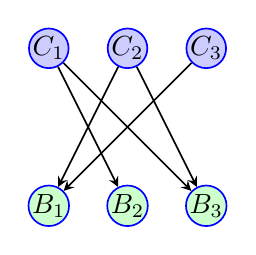
\begin{tikzpicture}[->, >=stealth, auto, semithick]
			% Set the positions of the nodes
			\node[circle, draw=blue, fill=blue!20, inner sep=0pt] (C1) at (0,0) {$C_1$};
			\node[circle, draw=blue, fill=blue!20, inner sep=0pt] (C2) at (1,0) {$C_2$};
			\node[circle, draw=blue, fill=blue!20, inner sep=0pt] (C3) at (+2,0) {$C_3$};
			\node[circle, draw=blue, fill=green!20, inner sep=0pt] (B1) at (0,-2) {$B_1$};
			\node[circle, draw=blue, fill=green!20, inner sep=0pt] (B2) at (1,-2) {$B_2$};
			\node[circle, draw=blue, fill=green!20, inner sep=0pt] (B3) at (2,-2) {$B_3$};
			% Draw the edges
			\draw (C1) to  (B2);
			\draw (C1) to  (B3);
			\draw (C2)to (B1);
			\draw (C2) to (B3);
			\draw (C3)to (B1);
		\end{tikzpicture}
		\caption{
			گراف اطلاعات جانبی برای
			\autoref{fig:fatemeh3}
		}
		\label{fig:fatemeh4}
	\end{figure}
\end{itemize}
\end{notation}
	\begin{remark}
	\label{remark:xbdiff}
	برای جلوگیری از گمراهی و ایجاد سردرگمی هر متغیر تصادفی و راس متناظر با آن به صورت معادل در ادبیات پژوهشی و این پایان‌نامه استفاده می‌شوند یعنی در هر بخش با توجه به این‌که در مورد گراف صحبت کنیم یا درباره‌ی متغیر تصادفی و توزیع آن،
    ممکن است از
	$X_i$
	یا
	$b_i$
	استفاده شود و به صورت صریح، تفاوتشان بیان نشود.
\end{remark}
 
	کدگذاری اندیس را می‌توان به صورت حالت خاصی از مسئله‌ی 	
	\transf{کدگذاری شبکه تک‌پخشی چندگانه}{multiple-unicast network coding}
 [رجوع شود به
	\cite{paper:Networkinformationflow}
	و
	\cite{yeung2008information}]
	در نظر گرفت. برای نمونه،
	\autoref{fig:fatemeh4}
	 را می‌توان به 
	 \autoref{fig:fatemeh5}
	  در نظر گرفت.
		\begin{figure}[H]
		\centering
		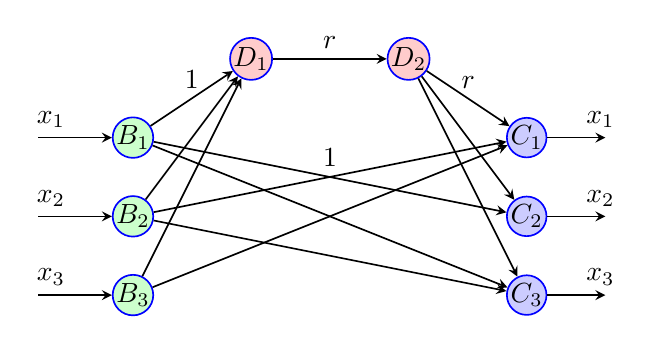
\begin{tikzpicture}[->, >=stealth, auto, semithick]
			% Set the positions of the nodes
			\node[circle, draw=blue, fill=red!20, inner sep=0pt] (D1) at (1.5,1) {$D_1$};
			\node[circle, draw=blue, fill=red!20, inner sep=0pt] (D2) at (3.5,1) {$D_2$};
			
			\node[circle, draw=blue, fill=blue!20, inner sep=0pt] (C1) at (5,0) {$C_1$};
			\node[circle, draw=blue, fill=blue!20, inner sep=0pt] (C2) at (5,-1) {$C_2$};
			\node[circle, draw=blue, fill=blue!20, inner sep=0pt] (C3) at (5,-2) {$C_3$};
			\node[circle, draw=blue, fill=green!20, inner sep=0pt] (B1) at (0,0) {$B_1$};
			\node[circle, draw=blue, fill=green!20, inner sep=0pt] (B2) at (0,-1) {$B_2$};
			\node[circle, draw=blue, fill=green!20, inner sep=0pt] (B3) at (0,-2) {$B_3$};
			% Draw the edges
			\draw (B1) to node[midway,above ] {$1$} (C2);
			\draw (B1) to(C3);
			\draw (B2)to (C1);
			\draw (B2) to(C3);
			\draw (B3)to (C1);
			\draw (D1)to node[midway,above ] {$r$} (D2);
			\draw (B1)to node[midway,above ] {$1$}(D1);\draw (B2)to (D1);\draw (B3)to (D1);
			\draw (D2)to node[midway,above ] {$r$}(C1);\draw (D2)to (C2);\draw (D2)to (C3);
			\draw (-1.2, 0)to node[midway,above left] {$x_1$} (B1) ;\draw (-1.2, -1)tonode[midway,above left] {$x_2$} (B2);\draw (-1.2, -2)tonode[midway,above left] {$x_3$} (B3);
			\draw (C1)to node[midway,above right] {$x_1$}(6,0) ;\draw (C2)to node[midway,above right] {$x_2$}(6, -1);\draw(C3) to node[midway,above right] {$x_3$}(6, -2);
		\end{tikzpicture}
		\caption{
			گراف اطلاعات جانبی برای 
			\autoref{fig:fatemeh3}
		}
		\label{fig:fatemeh5}
	\end{figure}
	ظرفیت یال‌های میانی و یال‌های ورودی به
	$D_1$
	برابر یک و ظرفیت یال
	$(D_1, D_2)$
	و یال‌های خروجی از
	$D_2$
	برابر
	$r$
	است که همان ظرفیت ارسال فرستنده است. برای توصیف دقیق مسئله‌ی کدگذاری شبکه و اثبات برابری آن با \icod به
	\cite{effros2012equivalence}
	رجوع کنید.
 
\begin{notation}
	به مسئله‌ی پیدا کردن کوتاه‌ترین اندیس‌کد برای 
 گراف\footnote{منظور از گراف در این پایان‌نامه گراف اطلاعات جانبی است، مگر این‌که صریحا خلاف آن گفته شود.}
	داده‌شده‌ی 
	$G$،
\\ \icodg 
	می‌گوییم.
\end{notation}
		\begin{remark}[پیرامون سختی \icod \cite{pliable2015paper}]
		تعداد نمونه‌های \icod با
		$n$
		پیام و 
		$n$
		گیرنده برابر
		$2^{n(n - 1)}$
		است. که برای
		$n$های
		کوچک نیز بسیار سریع رشد می‌کند. حتی حذف گراف‌های یک‌ریخت نیز تاثیری ندارد (برای مشاهده‌ی تعداد گراف‌های یک‌ریخت می‌توان به سایت \cite{web:unlabeled} مراجعه کرد.)
	
     مسئله‌ی
	\icod
نه تنها	
 \nphard  
 است،
 بلکه حتی پیدا کردن ضریب ثابتی از جواب هم سخت است. همچنین
	\namef{هویو}{Ishay Haviv}
	و
	\namef{لنبرگ}{Michael Langberg}
	در
	\cite{6283850}
	نشان داده‌اند، حتی زمانی که گراف اطلاعات جانبی تصادفی باشد، سایز کمینه‌ی یک کد خطی تقریبا همیشه
	$\Omega(\sqrt{n})$
	است.
		\end{remark}


\subsection{تاریخچه پژوهشی، کاربردها و ارتباط با دیگر مسائل ریاضی}
اولین بار
\icod توسط بیرک و کول 
\cite{25, 26}
 در زمینه‌ی ارتباطات ماهواره‌ای معرفی شد. فرمول‌بندی‌های مرتبط نیز پیشتر در کارهای 
 \namef{سلبیلر}{Celebiler}
 	و 
 	\namef{استت}{Stette}
  \cite{paper:1455117:Celebiler}،
  \namef{واینر}{A.D. Wyner}،
  \namef{ولف}{J.K. Wolf}
  و
  \namef{ویلمز}{F.M.J. Willems}
\cite{152}
و
\namef{یئونگ}{R.W. Yeung}
\cite{158}
 مورد مطالعه قرار گرفته است.
 
 \noindent
  اصطلاح "کدگذاری اندیس" را 
  \namef{بار-یوسف}{Bar-Yossef} 
  ، بیرک،
  \namef{جیرم}{T. S. Jayram}
  و کول در
\cite{4031356}
 برای اولین بار به کار برده‌اند. آن‌ها مسئله \icod را با مسئله کدگذاری منبع بدون خطا با اطلاعات جانبی که توسط
 \namef{ویتسنهاوزن}{H. Witsenhausen}
\cite{1055607}
 مطالعه شده است، مقایسه کرده و این نکته را مشخص کردند که در \icod، هدف گیرنده پیدا کردن بخشی از منبع است. در واقع گیرنده به دنبال یک اندیس است. پس، همانند کانال‌های ترکیبی
 \cite{27, 53, 154}،
 فرستنده می‌تواند به صورت پیش‌دستانه ارسال خود را کدگذاری کرده و برای گیرنده‌ها در تمامی پیکربندی‌های ممکن ارسال کند
\cite{48}.

 علاوه بر ارتباطات ماهواره‌ای، \icod در زمینه‌های متنوعی مانند توزیع چندرسانه‌ای 
\cite{114}،
مدیریت تداخل 
\cite{81}،
و کش‌های کدگذاری شده 
\cite{103, 82}
 کاربرد دارد. این مسئله همچنین به بسیاری از مسائل مهم دیگری مانند کدگذاری شبکه 
\cite{122, 61, 59}،
ذخیره‌سازی توزیع‌شده قابل بازیابی محلی 
\cite{108, 128, 13}،
بازی‌های حدس‌زنی روی گراف‌های جهت‌دار 
\cite{122, 162, 13}،
نظریه ماتروید 
\cite{61}،
و ظرفیت بدون خطای کانال‌ها 
\cite{131}
 نیز نزدیک است.
 
به خاطر این اهمیت، مسئله \icod به طور گسترده‌ای طی دو دهه گذشته مورد مطالعه قرار گرفته است. ابزارهای متنوعی از جمله نظریه گراف، نظریه کدگذاری، و نظریه اطلاعات برای ارائه طرح‌های کدگذاری غیر بدیهی
\cite{25, 101, 22, 43, 114, 29, 8, 104, 81, 130, 7, 9, 149, 116, 80, 141, 146, 162}
و همچنین کران‌‌های بالا و پایین 
\cite{160, 22, 55, 28, 17, 141}
 بکار رفته‌اند.
 
 یکی از مسیرهای پژوهشی، تعریف گونه‌های جدید برای مسئله است. برای مثال اگر گیرنده‌ها به جای این که به دنبال دریافت یکی از پیام‌ها باشند، به دنبال پیام جدیدی که جزو اطلاعات جانبی آن‌ها نیست باشند به کدگذاری اندیس منعطف می‌رسیم که موضوع اصلی این پایان‌نامه است. برای دیدن گونه‌های مختلف می‌توان به
 \cite{pliablefirstpaper, verypliable, byrne2023preferential}
 رجوع کرد.
 \pagebreak
 \section{کدگذاری اندیس منعطف}
 
 \subsection{معرفی}
 در مسئله‌ی
 \icod
 هر گیرنده به دنبال یازیابی یک پیام خاص است. در واقع در این صورت‌بندی هر گیرنده با کمک اطلاعات جانبی خود و اطلاعات دریافتی از فرستنده تلاش می‌کند پیامی را که از قبل به دنبال آن بوده است، بازیابی کند. اما اگر برای گیرنده ترجیحی بین پیام‌های مختلف نباشد چه باید کرد؟ در واقع اگر هدف گیرنده صرفا بازیابی پیامی باشد که از قبل در اطلاعات جانبی خود نداشته است به مسئله‌ی جدیدی می‌رسیم که آن را کدگذاری اندیس منعطف یه با اختصار \picod می‌نامیم. واژه منعطف در کدگذاری اندیس منعطف دقیقا به همین ویژگی گیرنده‌ها اشاره دارد که نسبت به حالت قبل شرایط کم‌تر سختگیرانه‌ای دارند.
 
 \picod توسط 
 \transf{براهما}{Siddhartha Brahma}
 و 
 \transf{فرگولی}{Christina Fragouli}
  در سال 2015 در
 \cite{pliablefirstpaper}
 به عنوان توسعه‌ای از \icod معرفی شد. در این صورت‌بندی علاوه بر این‌که فرستنده یک تابع کدگذاری انتخاب می‌کند، پیش از ارسال پیام و در هنگام انتخاب تابع کدگذاری، باید برای هر گیرنده بر اساس اطلاعات جانبی‌اش معین کند که چه پیامی را بازيابی خواهد کرد. پس از آن هر گیرنده بر اساس این انتخاب و مجموعه‌ی اطلاعات جانبی خودش، یک تابع کدگشایی انتخاب می‌:ند.
 
 با منعطف کردن گیرنده‌ها انتظار داریم که طول کد بهینه بهبود یابد. در 
 \autoref{chapter:literature}
 خواهیم دید که از کران خطی نسبت به تعداد گیرنده‌ها در
 \icod
 به کران لگاریتمی نسبت به تعداد گیرنده‌ها می‌رسیم که بهبود چشم‌گیری است.
 
 همان طور که قبلا بیان شد، هدف اصلی این پایان‌نامه بررسی
 \picod
 است. پیش از شروغ فصل‌های پیشرو و بررسی دقیق \picod، در ادامه این فصل به بررسی و دسته‌بندی مقالات حوزه‌ی
  \picod
  می‌پردازیم.
 \subsection{مروری اجمالی بر مقالات حوزه‌ی
 	\picod}
  پژوهش بر روی کدگذاری اندیس منعطف را می‌توان به چهار دسته‌ی زیر تقسیم کرد:
 \begin{enumerate}
 	\item 
 	ساخت یک کد برای دسته‌ای از گراف‌ها یا ساخت الگوریتم‌های تقریبی/تصادفی برای همه‌ی گراف‌ها
 	\item 
 	تعریف مسائل جدید بر پایه‌ی کدگذاری اندیس منعطف(مانند کدگذاری اندیس ترجیحی و \ldots)
 	\item 
 	استفاده از کدگذاری اندیس منعطف برای مدل‌سازی و حل مسائل دیگر
 	\item 
 	کران بالا برای حداکثر تعداد ارسال مورد نیاز و کران پایین برای حداقل تعداد ارسال مورد نیاز
 \end{enumerate}
 
 روی هرکدام از موضوعات بالا مقالات متعددی کار شده است. برای مثال
 \begin{enumerate}
 	\item الگوریتم‌/کد جدید
 	\begin{enumerate}
 		\item 
 		\namef{تانگ لیو}{Tang Liu}
 		 در
 		\cite{8278015}
 		با استفاده از روش‌های نظریه اطلاعات به اثبات کران‌هایی برای چند خانواده مختلف از گراف‌های اطلاعات جانبی می‌پردازد.
 		\item 
 		در
 		\cite{10313405}
 		الگوریتم حریضانه‌ی جدیدی بر پایه الگوریتم حریضانه‌ی فرگولی که در
   \autoref{algorithm:grcov}
   معرفی می‌کنیم ارائه می‌شود.
 		\item
 		در
 		\cite{8871209}
 		مسئله را فقط برای بخشی از گراف‌های اطلاعات جانبی که
 		\lr{complete–S PICOD}
 		نام‌گذاری می‌کنند، حل می‌کنند.
 		\item
 		در
 		\cite{9759449}
 		با تعریف یک مسئله‌ی
 		\transf{بهینه‌سازی تنک و با رنک پایین}{sparse and low-rank optimization}
 		و حل آن با 
 		\transf{الگوریتم تصویر کردن تکراری}{Alternating Projection Algorithm}
 		الگوریتمی کارا برای حل مسئله ارائه می‌دهند.
 		\item
 		در
 		\cite{8682270}
 		با استفاده از
 		\picod
 		و الگوریتم بر مبنای
 		\transf{تفاوت تحدب}{difference-of-convex}
 		ارائه می‌دهند که بر اساس نتایج آزمایشگاهی باعث کاهش پهنای باند مورد نیاز در
 		\transf{یادگیری توزیع شده روی دستگاه‌های نهایی}{ON-DEVICE DISTRIBUTED LEARNING}
 		می‌شود.
 		\item
 		در
 		\cite{sasi2019pliable}
 		برای کلاس خاصی از مسئله‌‌های
 		\picod
 		که
 		\transf{متوالی}{consecutive}
 		نامیده می‌شود بحث می‌کنند و برای دو حالت اکستریم آن اندیس‌کد ارائه می‌دهند. سپس در ادامه برای حالت
 		\lr{c-Constrained}
 		نیز کد ارائه می‌دهند.
 		\item 
 		در
 		\cite{8613483}
 		شبیه مقاله قبلی بر روی
 		\lr{Consecutive Complete–S}
 		کار می‌کنند و با استفاده از اثبات‌های ترکیبیاتی، اثباتی برای وجود کد با طول مناسب ارائه می‌دهند.
 	\end{enumerate}
 	\item گونه‌های جدید
 	\begin{enumerate}
 		\item
 		\namef{
 			یوچنگ لیو
 		}{Yucheng Liu}
 		 در
 		\cite{10015670}
 		به مسئله‌ی نشتی ناخواسته‌ی اطلاعات در
 		\icod
 		و
 		\picod
 		می‌پردازد. اگر بخشی از پیام‌ها حساس و بقیه غیرحساس باشند یک شنودکننده‌ی متخاصم بر اساس پیام‌های دریافتی چه مقدار داده کسب خواهد کرد؟ این مقدار را با
 		\transf{نرخ نشت}{leakage rate}
 		نشان می‌دهیم. در ادامه نرخ نشت بهینه برای مسائل
 		\icod
 	را اثبات می‌کنند و الگوریتم قطعی برای پیدا کردن آن ارائه داده و نشان می‌دهند نتیجه‌ی به‌دست‌آمده برای
 		\icod،
 		برای
 		\picod
 		هم برقرار است.
 		\item 
 		فرگولی در
 		\cite{6620405}
 		مسئله‌ی
 		\picod
 		را به دو روش تعمیم می‌دهد. در روش اول هر گیرنده به جای این‌که به دنبال بازیابی یک پیام باشد به دنبال بازیابی
 		$t$
 		پیام است که به آن
 		\lr{MULT-PICOD}
 		می‌گوید.
 		در روش دوم فرستنده، گراف اطلاعات جالبی را در دست ندارد و تنها می‌داند که گیرنده‌ها چند پیام را از پیش، به عنوان اطلاعات جانبی دارند(همه‌ی گیرنده‌ها به تعداد برابر پیام دارند.) و آن را
 		\lr{OB-PICOD}
 		می‌نامد.
 		\item 
 		\namef{سانگ}{Linqi Song}
 		 کار فرگولی در مقاله قبلی را در
 		\cite{8625330}
 		ادامه می‌دهد و روش کدگذاری جدیدی برای 
 		\lr{MULT-PICOD}
 		ارائه می‌دهد.
 		\item 
 		لیو در
 		\cite{9173957}
 		گونه جدیدی از مسئله را تعریف می‌کند که اولا به جای وجود سرور مرکزی، تبادل پیام به صورت نامتمرکز انجام می‌شود و همچنین هر گیرنده تنها یک پیام جدید خارج از اطلاعات جانبی خود بازیابی می‌کند و هیچ دیتایی راجع به بقیه پیام‌ها کسب نمی‌کند. به دلیل سختی این مسئله، در ادامه تنها روی یک حالت خاص که اطلاعات جانبی گیرنده‌های به صورت
 		\transf{جابه‌جایی‌های چرخشی 
 			$s$تایی}{$s$ circular shifts}
 		هست تمرکز می‌کنند.	
 		
 	\end{enumerate}
 	\item حل مسائل دیگر
 	\begin{enumerate}
 		\item 
 		در
 		\cite{Obead_2023}
 		با استفاده از  
 		\picod
 		مسئله‌ی
 		\transf{بازیابی منعطف و محرمانه‌ی دیتا، همراه با اطلاعات جانبی با یک سرور}{Single-Server Pliable Private Information Retrieval With Side Information}
 		را حل می‌کنند.
 		\item
 		سانگ و فرگولی در
 		\cite{8404065}
 		به ارتباط 
 		\picod
 		و ساختن سیستم‌های پیشنهاددهنده‌ با توجه به پهنای باند می‌پردازند.
 		\item
 		در
 		\cite{e24081149}
 		به ارتباط 
 		\icod
 		و
 		\picod
 		کدهای تصحیح خطا با تفسیرهای متعدد از ساختار درختی کدهای چرخه‌ای تو در تو
 		\lrfootnote{error-correcting codes with multiple interpretations from the tree construction of nested cyclic codes}
 		می‌پردازند.
 		\item 
 		فرگولی در
 		\cite{datashuf}
 		با استفاده از
 		\picod
 		به مسئله‌ی
 		\transf{بازآرایی داده}{Data Shuffling}
 		که در مسائل محاسبه‌ی توزیع‌شده ظاهر می‌شود، می‌پردازد.
 		\item
 		سانگ و فرگولی در
 		\cite{7176784}
 		یک بررسی‌ اجمالی بر تاثیر ایده‌ی فکری پشت
 		\picod
 		بر دسته‌ای از مسائل مخابراتی که
 		\transf{کدگذاری نوع محتوا}{Content-Type Coding}
 		نامیده می‌شود می‌پردازند. سانگ در ادامه در پایان‌نامه‌ی دکتری خود
 		\cite{linqiphd}
 		نتایج متعددی در این زمینه ثابت می‌کند.
 	\end{enumerate}
 	\item کران بالا و پایین
 	\begin{enumerate}
 		\item 
 		کران بالای
 		$\mathcal{O}(\log(n))$
 		برای
 		\picod
 		با کران بالای
 		\icod
 		که
 		$\mathcal{O}(n)$
 		است تفاوت فاحشی دارد. لیو و تانینتی در
 		\cite{7606849}
 		تلاش می‌کنند با پیدا کردن کرانی برای تعداد گیرنده‌هایی که با هر پیام می‌توان ارضا کرد شهودی برای این مسئله بیابند.
 		\item 
 		در
 		\cite{9518120}
 		گراف اطلاعات جانبی را با استفاده از 
 		\transf{هایپرگراف‌ها}{hyper graphs}
 		مدل‌سازی کرده و کران بالایی برای تعداد ارسال‌ها پیدا می‌کنند. سپس با استفاده از این کران اثبات می‌کنند که برای بعضی از حالت‌ها کد با طول خوبی وجود دارد.
 		\item
 		در ادامه مقاله قبل با روش مشابهی در
 		\cite{9965883}
 		کران بالا و کران پایین برای
 		\picod
 		اثبات شده است.
 		\item
 		\transf{انگ}{ong}
 		و همکاران در
 		\cite{ong2019improved}
 		و سپس در
 		\cite{8849527}
 		تکنیک بسیار متفاوتی در پیش می‌گیرند. به جای بررسی اطلاعات جانبی گیرنده‌ها به 
 		\transf{گیرنده‌های غایب}{Absent Receivers}
 		می‌پردازند. اگر هر گیرنده را بر اساس اطلاعات جانبی‌اش شناسایی کنیم، به زیرمجموعه‌های مجموعه‌ی پیام‌ها که به عنوان گیرنده در گراف وجود ندارند گیرنده‌ی غایب می‌گوییم. با استفاده از این روش، کران پایین جدیدی برای حداقل ارسال مورد نیاز پیدا می‌کنند.
 	\end{enumerate}
 \end{enumerate}
 
\pagebreak 
\section{اهداف و دست‌آورد‌های پژوهشی}
از نظر پژوهش ریاضی در زمینه‌ی \picod بخش عمده‌ی کارها به یافتن کران بالایی برای تعداد پیام مورد نیاز روی گراف‌های مختلف صورت گرفته است. به طور خاص در کدگذاری اندیس منعطف به این مسئله تشدید نیز می‌شود و تقریبا کار پژوهشی‌ مهمی روی کران پایین انجام نشده است. هدف اولیه شروع این پژوهش‌، تکمیل این بخش از پژوهش‌ها با یافتن کران پایین برای \picod بود.
%shit
\section{ساختار پایان‌نامه}

این پایان‌نامه در شش فصل به شرح زیر ارائه می‌شود.

فصل دوم به بیان پیش‌نیازهای علمی مورد نیاز، شامل مطالبی پیرامون نظریه گراف، نظریه اطلاعات، جبرخطی و روش‌های احتمالاتی می‌پردازد.

فصل سوم به مطالعه و بررسی کارهای پیشین با موضوع این پایان‌نامه می‌پردازد. در این فصل به کارهای بنیادی فرگولی در زمینه‌ی کدگذاری اندیس منعطف می‌پردازیم و یک الگوریتم چندجمله‌ای قطعی برای مسئله را بررسی می‌کنیم.

در فصل چهارم، به گونه‌های مختلف مسئله می‌پردازیم و با مقدمات و کاربردهای هرکدام آشنا می‌شویم.

در فصل پنجم، نتایج جدیدی که در این پایان‌نامه به‌دست آمده است، ارائه می‌شود.

در فصل ششم به جمع‌بندی کارهای انجام‌شده در این پژوهش و ارائه‌ی پیشنهادهایی برای انجام کارهای آتی پرداخته می‌شود.